\documentclass[11pt]{article}

% ---------- 中文支持 ----------
\usepackage{iftex}
\ifXeTeX
  \usepackage{fontspec}
  \usepackage{xeCJK}
  \defaultfontfeatures{Ligatures=TeX}
  \setmainfont{Times New Roman}
  \IfFontExistsTF{Songti SC}{
    \setCJKmainfont{Songti SC}
  }{
    \IfFontExistsTF{STSong}{
      \setCJKmainfont{STSong}
    }{
      \setCJKmainfont{PingFang SC}
    }
  }
\else
  \usepackage[utf8]{inputenc}
  \usepackage[T1]{fontenc}
\fi

\usepackage{PRIMEarxiv}
\usepackage{geometry}
\usepackage{amsmath,amssymb}
\usepackage{graphicx}
\usepackage{multirow}
\usepackage{booktabs}
\usepackage{hyperref}
\usepackage{subcaption}
\usepackage{authblk}
\usepackage{array}
\pagestyle{fancy}
\thispagestyle{empty}
\rhead{ \textit{ }}

\usepackage{listings}
\usepackage[dvipsnames]{xcolor}

% Define Python styling
\lstset{
    language=Python,
    basicstyle=\ttfamily\small,
    keywordstyle=\color{blue},
    stringstyle=\color{blue},
    commentstyle=\color{ForestGreen},
    numbers=left,
    numberstyle=\tiny\color{gray},
    stepnumber=1,
    numbersep=5pt,
    backgroundcolor=\color{white},
    showspaces=false,
    showstringspaces=false,
    frame=single,
    rulecolor=\color{black},
    breaklines=true
}

\usepackage{fancyhdr}
\usepackage{adjustbox}

\pagestyle{fancy}
\renewcommand{\headrulewidth}{0.65pt}
\setlength{\headsep}{1.3cm}

\lhead{}

\fancypagestyle{firstpage}{
  \fancyhead{}
  \lhead{
      \adjustbox{valign=m}{
\includegraphics[height=0.9cm]{logo/huawei.png}}
      \hspace{1em}
      \adjustbox{valign=m}{
\includegraphics[height=0.86cm]{logo/hkustgz.png}}
      \hspace{1em}
      \adjustbox{valign=m}{
\includegraphics[height=0.9cm]{logo/hkust.png}}
  }
  \renewcommand{\headrulewidth}{0.65pt}
  \setlength{\headsep}{1.3cm}
}

\title{HyperParallel：一种超节点亲和性AI框架\footnote{贡献者完整列表见论文末尾的致谢章节。}}
\author[$\dagger$]{Xin Zhang}
\author[$\ddagger$]{Beilei Sun}
\author[$\ddagger$]{Teng Su}
\author[$\ddagger$]{Qinghua Zhang}
\author[$\ddagger$]{Chong Bao}
\author[$\dagger$]{\\Lei Chen}
\author[$\ddagger$]{Xuefeng Jin}

\affil[$\dagger$]{\textit{香港科技大学 \& 香港科技大学（广州），香港及广州，中国}}
\affil[$\ddagger$]{\textit{华为技术有限公司，中国}}

\date{}

\begin{document}
\maketitle

\thispagestyle{firstpage}

\begingroup
\renewcommand\thefootnote{*}
\footnotetext{贡献者完整列表见论文末尾的致谢章节。}
\endgroup

\begin{abstract}
大规模、稀疏、多模态和智能体AI模型的涌现，与硬件向超节点架构的转变同步发生。超节点架构将数百乃至数千个加速器通过超低延迟互联和统一内存池集成在一起。然而，现有的AI框架并未设计为高效利用这些架构，导致编程复杂度高、负载不均衡以及内存利用率低等问题。本文提出了一种超节点亲和性AI框架，将超节点视为单一逻辑计算机，并将硬件感知的编排嵌入到框架中。在MindSpore中实现的HyperParallel架构包含三个核心组件：用于自动分层内存管理的HyperOffload、用于跨异构工作负载细粒度MPMD并行的HyperMPMD，以及用于声明式并行策略规范的HyperShard。这些技术协同作用，在降低并行编程和系统调优开销的同时，显著提升了训练和推理效率，证明了超节点亲和性对下一代AI框架的必要性。
\end{abstract}

\section{引言}
人工智能的快速进步由模型架构、训练范式和硬件系统的协同演进推动~\cite{mudigere2022software,pandey2019machine, paszke2019pytorch}。现代基础模型在参数规模~\cite{fedus2022switch,hoffmann2022training,ren2023pangu}和功能范围上持续扩展，从纯语言系统扩展到多模态~\cite{sun2024generative}、稀疏~\cite{chen2022towards,dettmers2023spqr}和智能体架构~\cite{yu2025dapo}。这些模型在计算负载上引入了显著的异构性、不规则的数据路由，以及对内存和通信带宽的海量需求。与此同时，硬件架构已演进为超节点集成集群——数千个加速器通过超低延迟的点对点互联和统一内存池相连~\cite{li2023pond,ubmesh,matrix384}。在这一背景下，AI框架作为关键的中间件层，成为连接高层算法抽象与日益复杂的硬件架构的桥梁。

我们发现，现有AI框架面临着\textit{性能-可编程性}鸿沟。传统的单程序多数据（SPMD）范式~\cite{darema2001spmd}难以处理专家混合（MoE）~\cite{chen2022towards,dettmers2023spqr}和多模态架构固有的负载不均衡问题。此外，跨分层内存层手动管理中间状态（权重、激活值和KV缓存）给研究人员带来了沉重的工程负担。现有的系统扩展层~\cite{barham2022pathways,jax2018github,jiang2024megascale,jung2025hlx,rasley2020deepspeed,ren2021zero,shoeybi2019megatron}虽在特定领域有效，但往往导致模型逻辑与硬件拓扑的紧密耦合，代码可移植性差，集群利用率也不理想。

这些挑战表明，仅对现有框架进行增量优化已不足够。相反，AI框架必须经历一次以明确拥抱超节点特性、重新思考并行性、内存和执行抽象为核心的架构转变。本文主张，超节点亲和性应成为下一代AI框架的核心设计原则。超节点亲和性框架将超节点视为单一的、逻辑统一的计算实体，并将硬件感知的编排直接嵌入框架运行时和编译器中。这样既能屏蔽算法开发者的底层系统复杂性，又能系统性地挖掘现代硬件的性能潜力。

基于这一洞见，我们提出了超节点亲和性AI框架，并在MindSpore中展示了其设计与实现。该框架引入了新颖的HyperParallel架构，整合三个核心组件：HyperOffload——通过统一内存池和自动卸载实现计算与模型状态的解耦；HyperMPMD——将并行执行从SPMD扩展到细粒度的多程序多数据（MPMD），以处理异构的多任务工作负载；HyperShard——提供将算法逻辑与并行策略设计解耦的声明式并行编程接口。这些组件共同为超节点集群上的MoE、全模态和强化学习工作负载提供灵活、高效的执行能力。

本文做出以下贡献：
\begin{itemize}
    \item \textbf{新兴挑战的系统性分析}：我们分析了模型工作负载、硬件架构和训练-推理范式的最新趋势，并识别了它们在超节点部署时对现有AI框架的根本性限制。
    \item \textbf{超节点亲和性框架设计}：我们提出了一种新的架构范式，将超节点视为"巨型计算机"，在框架内抽象复杂的网络拓扑、分层内存系统和异构执行环境。
    \item \textbf{HyperParallel架构}：我们引入并实现了HyperOffload、HyperMPMD和HyperShard，实现统一的状态管理、灵活的MPMD并行以及声明式并行编程。
    \item \textbf{实证验证}：我们证明了所提框架在代表性大规模工作负载上显著提升了训练和推理效率，同时降低了开发和优化开销，验证了其有效性。
\end{itemize}

本文其余部分组织如下：第~\ref{sec2}节刻画了模型和硬件的演进，回顾了现有AI框架，并分析了万亿参数LLM时代AI框架所面临的挑战。第~\ref{sec4}节介绍了所提超节点亲和性框架的设计和关键技术。第~\ref{sec5}节以对结果的讨论和未来方向作结。

\section{背景}
\label{sec2}

AI框架作为关键的中间件层，位于模型算法和底层硬件架构之间，是加速整个人工智能领域进步的基础软件基础设施。其演进本质上由算法复杂性和硬件创新的双重需求驱动。一方面，框架必须提供高层次抽象，使研究人员能够高效地开发、调试和验证新颖的架构，从而促进快速的算法迭代。另一方面，它必须系统地将这些高层次抽象转化为最大化硬件利用率、充分挖掘专用计算资源潜力的优化可执行程序。

\subsection{小型深度学习模型时代}

\textbf{模型与硬件。}在深度学习的早期阶段，大多数模型体量较小。例如，小规模的计算机视觉（CV）模型~\cite{zhao2024review}通常可以放入单个加速器的内存中。参数量适中的自然语言处理（NLP）模型~\cite{liu2019roberta}虽然超出了单卡内存容量，但通常可以在具有多个GPU的单台机器上运行。

\noindent \textbf{训练范式。}训练小型深度学习模型时，CV模型的主要训练策略是数据并行（DP），单卡计算能力是主要性能瓶颈。对于中等规模的NLP模型，通常采用模型并行将组件分片到节点内的多张卡上。较高的节点内通信量使内部带宽成为关键瓶颈。

\noindent \textbf{AI框架。}为了在单台机器上处理此类工作负载，PyTorch~\cite{paszke2019pytorch}凭借高度的执行灵活性成为主导生态系统。PyTorch的核心优势在于其动态计算图和丰富的生态系统，使其非常适合快速原型设计、模型定制和学术研究。

\subsection{十亿规模大型语言模型时代}

\noindent \textbf{模型与硬件。}随着大型语言模型的出现，模型参数量迅速扩展到数千亿。海量预训练数据集对硬件也提出了更高要求。通常在训练十亿规模LLM时需要构建包含多节点的服务器集群。

\noindent \textbf{训练范式。}预训练和监督微调是十亿规模LLM最常见的两种训练任务。多维分片（数据并行、张量并行和流水线并行）策略被广泛采用。不同的分片策略对集群带宽提出了不同的需求。特别是张量并行（TP）、流水线并行（PP）和上下文并行（CP）需要频繁的跨服务器通信——每次传输通常超过数GB——这很难通过计算-通信重叠来隐藏。例如，在典型的训练设置中，TP的数据流量开销占训练时间的52.9\%~\cite{ubmesh}。因此，跨机通信成为主要性能瓶颈，导致集群资源利用率不理想。

\noindent \textbf{AI框架。}PyTorch的主要局限性包括缺乏全面的多程序多数据（MPMD）能力，以及缺乏对计算与存储解聚的原生支持。为解决这些瓶颈，许多框架应运而生，如JAX~\cite{jax2018github}、DeepSpeed~\cite{rasley2020deepspeed}、Megatron~\cite{shoeybi2019megatron}和HLX~\cite{jung2025hlx}，作为专用系统扩展层。这些框架专注于分布式策略、内存优化、并行拓扑、混合注意力兼容性和高效多模态处理。

\begin{itemize}
    \item \textbf{JAX：函数式编程与编译器驱动的加速} -- JAX利用函数式编程范式结合可组合的变换（\textit{jit, pmap, vmap}），使编译器能够跨算子、并行性和微分执行统一优化。它在大规模TPU训练、科学计算以及需要精确控制计算图变换的研究中表现出色。然而，其生态系统高度专业化，导致编程复杂度较高。
    
    \item \textbf{DeepSpeed：大规模训练的系统工具箱} -- DeepSpeed提供ZeRO系列冗余消除分片、MoE优化器、高效通信和卸载支持，是在受限GPU资源下训练超大模型的关键基础设施。它作为系统增强层与PyTorch紧密集成，以弥补内存效率和分布式调度方面的不足。一个重大缺陷是其假设网络拓扑相对均匀；而在实际超节点中，机架间延迟和带宽差异极大，DeepSpeed对SPMD和静态分片的依赖可能导致严重的负载不均衡和硬件利用率低下。
    
    \item \textbf{Megatron：密集与稀疏模型的极致并行} -- Megatron强调流水线并行、张量并行和MoE并行的优化，以实现峰值的分布式性能。其"规模优先"的设计哲学非常适合在GPU资源充足的环境中追求最大吞吐量。尽管Megatron-Core正在演进为LLM训练的基础模块，但该框架存在通信逻辑与硬件拓扑紧密耦合的问题，导致代码可移植性差、编程复杂度高，参数调优和性能优化成本高昂。

    \item \textbf{HLX：混合注意力架构的加速} -- HLX专为具有线性和全局混合注意力的新型Transformer变体设计。它引入多线程并行编排和双维（行/列）计算流水线，以加速稀疏和线性注意力算子。通过深度整合算子结构与线程调度，HLX为混合注意力模型提供了系统级加速方案。然而，它缺乏框架级的超节点统一内存池管理，迫使研究人员手动管理训练和推理的中间状态。
\end{itemize}

\noindent \textbf{相关研究工作。}除上述框架外，还有一些研究工作解决了LLM预训练整个生命周期中的其他瓶颈。

\begin{itemize}
    \item \textbf{集群级容错与算法-系统协同设计} -- {MegaScale}~\cite{jiang2024megascale}代表了集群级训练基础设施的发展趋势。在跨多节点的大规模分布式算力环境中，它通过算法/内核优化、3D并行通信重叠和自动故障监控，在万卡集群上实现了较高的模型FLOP利用率（MFU）。然而，实现有效的计算-通信重叠需要高度定制的并行策略和代码实现，导致调试和迁移成本极高。
    
    \item \textbf{中大规模训练的分片与卸载} -- 以\textit{ZeRO}生态系统（特别是ZeRO-3和ZeRO-Offload）~\cite{rajbhandari2020zero, ren2021zero}为代表，该方向针对数百亿到数万亿参数的模型训练。核心方法是在GPU集群间对参数、梯度和优化器状态进行全分片，通常结合CPU/NVMe卸载来打破GPU内存墙。这些方法利用高效的通信分区实现近线性扩展。然而，它们依赖静态内存分区，缺乏统一内存池的自动管理能力，可能导致内存碎片化。
    
    \item \textbf{超大规模加速器集群的调度与通用执行层} -- \textit{Pathways}~\cite{barham2022pathways}展示了超大规模集群统一执行层的必要性。该方向专注于跨加速器Pod的异步数据流、调度和拓扑优化，以实现流水线并行、数据并行和模型并行之间的无缝协作。与传统的刚性SPMD模型不同，它支持MoE模型所必需的细粒度、不规则路由。然而，其对中心化资源管理器和协调器的依赖，可能在跨异构节点管理高度动态的大规模任务图时引入调度开销和延迟瓶颈。
    
\end{itemize}

\subsection{万亿规模大型语言模型时代}

\noindent \textbf{模型。}近期，主流大型语言模型在规模、架构和目标模态上出现了重大变化。具体而言，最先进的LLM通常拥有万亿级参数，并利用专家混合（MoE）架构在扩展参数的同时增加稀疏性，对文本以外多种模态的支持也日益普及。

\begin{itemize}
    \item 从模型规模和架构角度看，许多最先进的LLM，如DeepSeek-V3~\cite{liu2024deepseek}和Qwen-3~\cite{yang2025qwen3}，利用MoE架构在扩展参数时增加稀疏性。这种方法在保持每token常数计算成本的同时扩展了模型容量并增强了泛化能力。
    \item 从纯语言模型到全模态系统的过渡在新发布的模型中日益普遍。这一过渡需要集成多样化的子模块，导致模型结构日趋不规则，使并行编程和优化都更加复杂。全模态模型通常采用多编码器、模态融合层、多解码器架构。多模态的桥接引入了模块级异构性和动态路由负载。
\end{itemize}

\noindent \textbf{训练范式。}训练范式从传统预训练转变为智能体强化学习（RL）。这一转变需要协同部署多种任务，包括训练、推理和智能体执行。这种异构化趋势对多任务、多模型工作流的编排提出了更严格的要求。具体地，为增强指令遵循、深度推理和复杂问题解决能力，最先进的大模型在初始预训练阶段后越来越多地引入RL。强化学习将工作负载范式从纯静态数据集训练转变为涉及动态数据的"采样-评估-更新"异构任务。这一工作流通常依赖大规模的rollout操作和异步的actor-learner架构，训练和推理任务并发执行。因此，底层框架必须支持强健的异构任务管理、异步任务调度以及针对多任务、多模型环境定制的动态编排能力。

\noindent \textbf{硬件特性。}超节点集群专为训练具有MoE、多模态和智能体特性的LLM而设计。以华为Matrix384~\cite{matrix384}（Atlas 900）超节点为例，我们分析超节点集群的典型特性：

\begin{itemize}
    \item \textbf{统一内存寻址与点对点架构} -- 基于UB互联协议（灵驱），系统将384个Ascend 910C NPU和192个鲲鹏CPU集成到单个超节点中。计算、内存和网络资源被解聚为独立的池化单元。
    \item \textbf{极高带宽与超低延迟} -- 传统架构依赖PCIe或以太网进行互联。Ascend 384超节点采用高效协议，与传统服务器架构相比通信带宽提升15倍，单跳延迟从2$\mu$s降至200ns——提升了十倍。
    \item \textbf{分层多样化的网络拓扑} -- 单个Ascend超节点的规模预计将从384卡增加到8192卡，未来目标达到15488卡。为支持这种大规模可扩展互联，超节点采用分层拓扑：每个机架内建立2D全连接网格，然后跨机架扩展为另一个2D全连接网格，最终形成4D全互联（全网格）拓扑。
\end{itemize}

\noindent \textbf{AI框架面临的挑战。}超节点为快速增长的模型参数和日益复杂的架构提供了优越的解决方案，但充分发挥其潜力需要应对若干根本性挑战。为降低算法开发和调优的复杂性，同时最大化大规模训练和推理效率，AI框架面临以下关键挑战：

\begin{table}[htbp]
\centering
\begin{minipage}{0.45\textwidth}
\centering
\caption{按模型类型的并行策略}
\begin{tabular}{ll}
\toprule
\textbf{模型 \& 算法} & \textbf{策略} \\
\midrule
\midrule
密集Transformer & DP, PP, TP, SP \\
\hline
稀疏MoE & DP, PP, TP, SP, EP \\
\hline
扩散模型 & DP, FSDP \\
\hline
长序列 & SP, CP \\
\hline
强化学习 & MPMD \\
\hline
$\cdots$ & $\cdots$ \\
\bottomrule
\end{tabular}
\label{table:Strategies_by_model}
\end{minipage}
\hfill
\begin{minipage}{0.53\textwidth}
\centering
\caption{按集群类型的并行策略}
\begin{tabular}{p{2.6cm}p{3.7cm}}
\toprule
\textbf{集群} & \textbf{策略} \\
\midrule
\midrule
单机\newline（8 DIE）& TP8，\newline PP负责其余 \\
\hline
单机（16 DIE）& 高维TP\newline（TP16），减少PP \\
\hline
8k节点\newline 超平面 & 拓扑感知TP16，\newline 减少PP \\
\bottomrule
\end{tabular}
\label{table:Strategies_by_cluster}
\end{minipage}
\end{table}

\begin{figure}
    \centering
    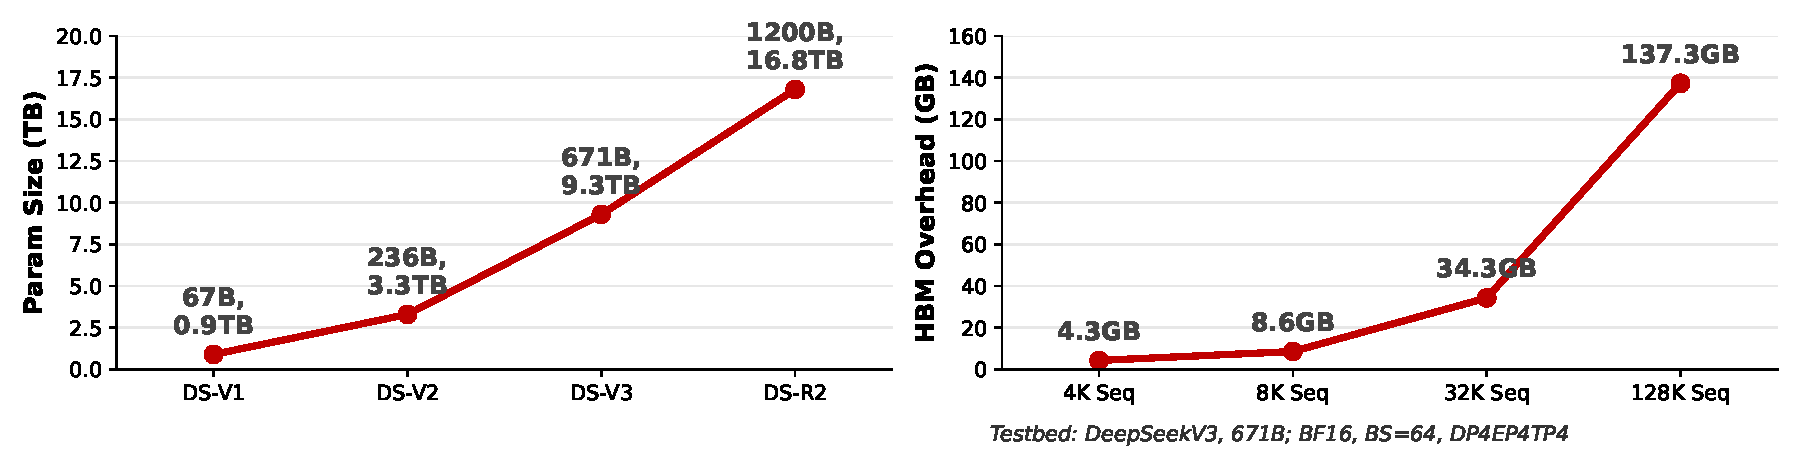
\includegraphics[width=\linewidth]{figures/intermediates.pdf}
    \caption{在模型训练和推理过程中，存储和管理参数及中间状态的复杂性持续增加。}
    \label{fig:intermediates}
\end{figure}

\begin{itemize}
    \item \textbf{挑战1：抽象复杂网络拓扑以简化并行编程} -- 随着超节点消除节点间带宽瓶颈，集群规模可增长至10万卡级别。驾驭如此复杂的网络拓扑需要精心设计和优化的并行策略。模型架构或集群配置的任何变化都需要完全重新设计这些策略，如表~\ref{table:Strategies_by_model}和表~\ref{table:Strategies_by_cluster}的示例所示。经验上，每次适配和调优周期需要高级系统优化工程师1--2周的工作量，并消耗大量集群资源，导致运营效率低下。
    
    \item \textbf{挑战2：实现灵活细粒度的并行性以最大化硬件利用率} -- 当前的并行分片主要依赖SPMD范式。然而，随着模型向MoE和全模态架构演进，不同模块和层呈现异构的计算负载。标准SPMD方法频繁导致负载不均衡；例如，在子模块负载各异的全模态模型中，SPMD结合流水线并行（PP）往往引发显著的流水线气泡。此外，MoE模型遭受高通信开销；在DeepSeek-V3中，专家并行（EP）通信占执行时间的17\%，通信掩盖率仅为61\%，远低于90\%的理想目标。
    
    \item \textbf{挑战3：通过内存池化管理中间状态以优化内存利用率} -- 随着模型规模从数千亿向数十万亿参数发展，管理中间状态（包括权重、激活值和KV缓存）的复杂性呈指数级增加。超节点通过内存语义互联提供统一的DRAM内存池。为保持性能，中间状态必须在使用前主动预取（换入）到高带宽存储器（HBM）中，以避免内存访问延迟。手动管理这些交换操作给算法研究人员带来了沉重的编程和优化负担。
\end{itemize}

\section{超节点亲和性AI框架的设计}
\label{sec4}
当前工业界训练和推理软件的优化工作不足以根本解决超节点对AI框架带来的系统性挑战。为充分利用超节点的优势并解决模型演进带来的瓶颈，AI框架必须以\textit{超节点亲和性}为核心进行架构重设计。通过整合超节点的特定架构特性，框架可以为研究人员提供变革性的编程体验，同时显著提升训练和推理效率。本章以MindSpore的实际实现为基础，介绍超节点亲和性AI框架的架构设计和关键技术。

\subsection{总体设计}

\begin{figure}
    \centering
    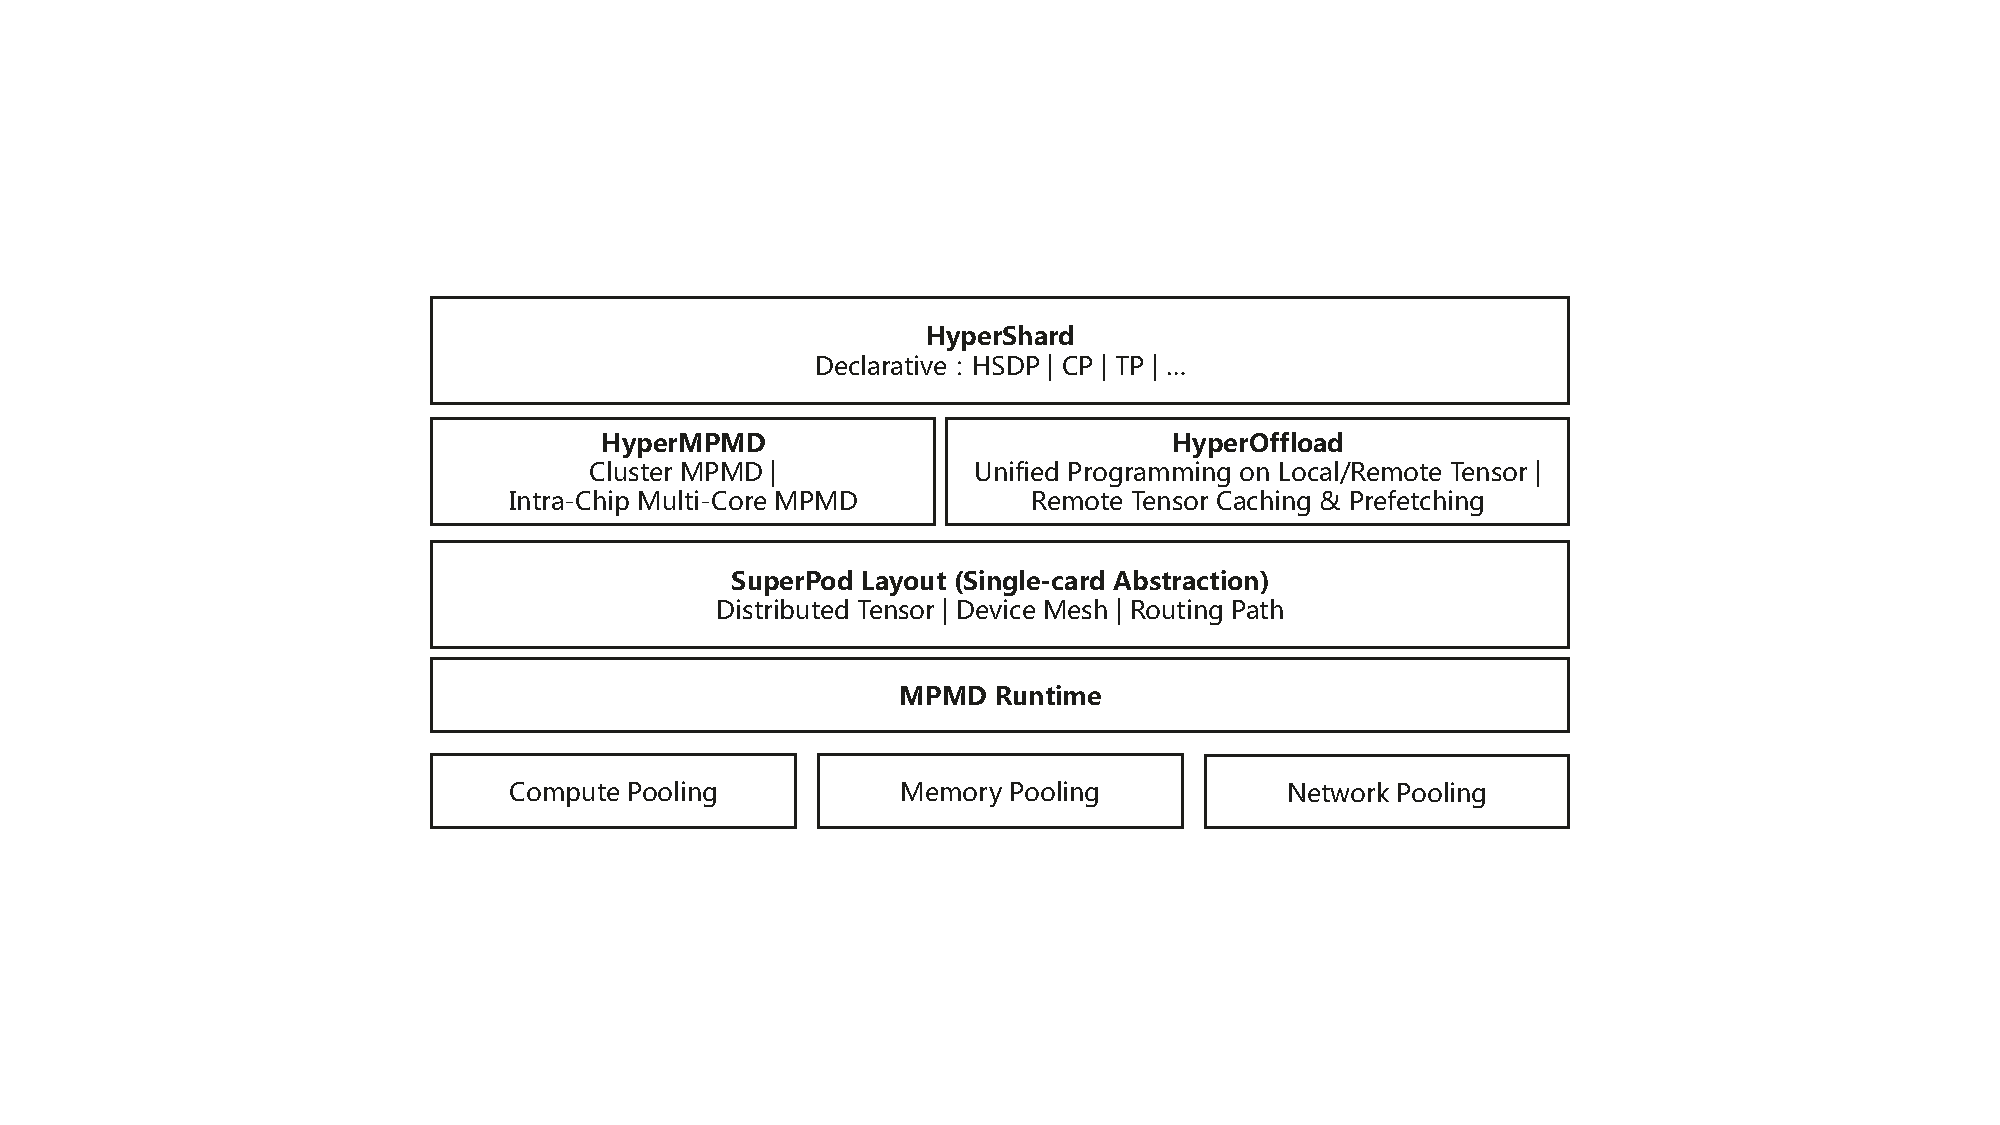
\includegraphics[width=0.9\linewidth]{figures/hyperparallel.pdf}
    \caption{\textit{HyperParallel}总体设计。}
    \label{fig:overall}
\end{figure}

MindSpore超节点亲和性的核心理念是通过AI框架抽象底层硬件复杂性，将超节点视为单一的"巨型计算机"。这种方法为算法研究人员提供了类似单节点系统的编程和执行体验。通过将复杂的软件工程任务（如并行分片和训练-推理状态管理）直接嵌入框架，MindSpore利用超节点的点对点架构优势，解决MoE、全模态和强化学习等复杂场景中的性能瓶颈。为此，我们提出如图~\ref{fig:overall}所示的\textbf{HyperParallel}架构，包含三个关键组件，旨在屏蔽用户的硬件复杂性，同时最大化架构优势：

\begin{itemize}
    \item \textbf{HyperOffload} -- 促进计算与状态的解耦。利用超节点的池化存储能力，解决不断增加的模型规模带来的内存瓶颈。
    \item \textbf{HyperMPMD} -- 将并行分片从传统的SPMD范式过渡到细粒度的多程序多数据（MPMD）方法。利用点对点计算架构，为强化学习和全模态工作负载提供灵活的并行性。
    \item \textbf{HyperShard} -- 推动从命令式到声明式编程的转变。它抽象超节点集群的复杂拓扑，为全模态和其他高级模型提供简约、可组合的编程体验。
\end{itemize}

在MindSpore上进行超节点模型开发、训练和推理的工作流程如下：

\begin{itemize}
    \item \textbf{步骤1：算法开发} -- 研究人员通过框架开发算法，利用HyperShard的声明式编程接口配置模型的并行策略。
    \item \textbf{步骤2：灵活并行} -- HyperMPMD以MPMD格式执行灵活、细粒度的并行，针对算法和集群的独特拓扑进行专门优化。
    \item \textbf{步骤3：运行时编排} -- 执行过程中，HyperOffload对计算、存储和网络进行全局编排，管理HBM与DRAM之间的状态交换，以充分利用超节点的分层内存池。
\end{itemize}

\subsection{HyperOffload}

\begin{figure}
    \centering
    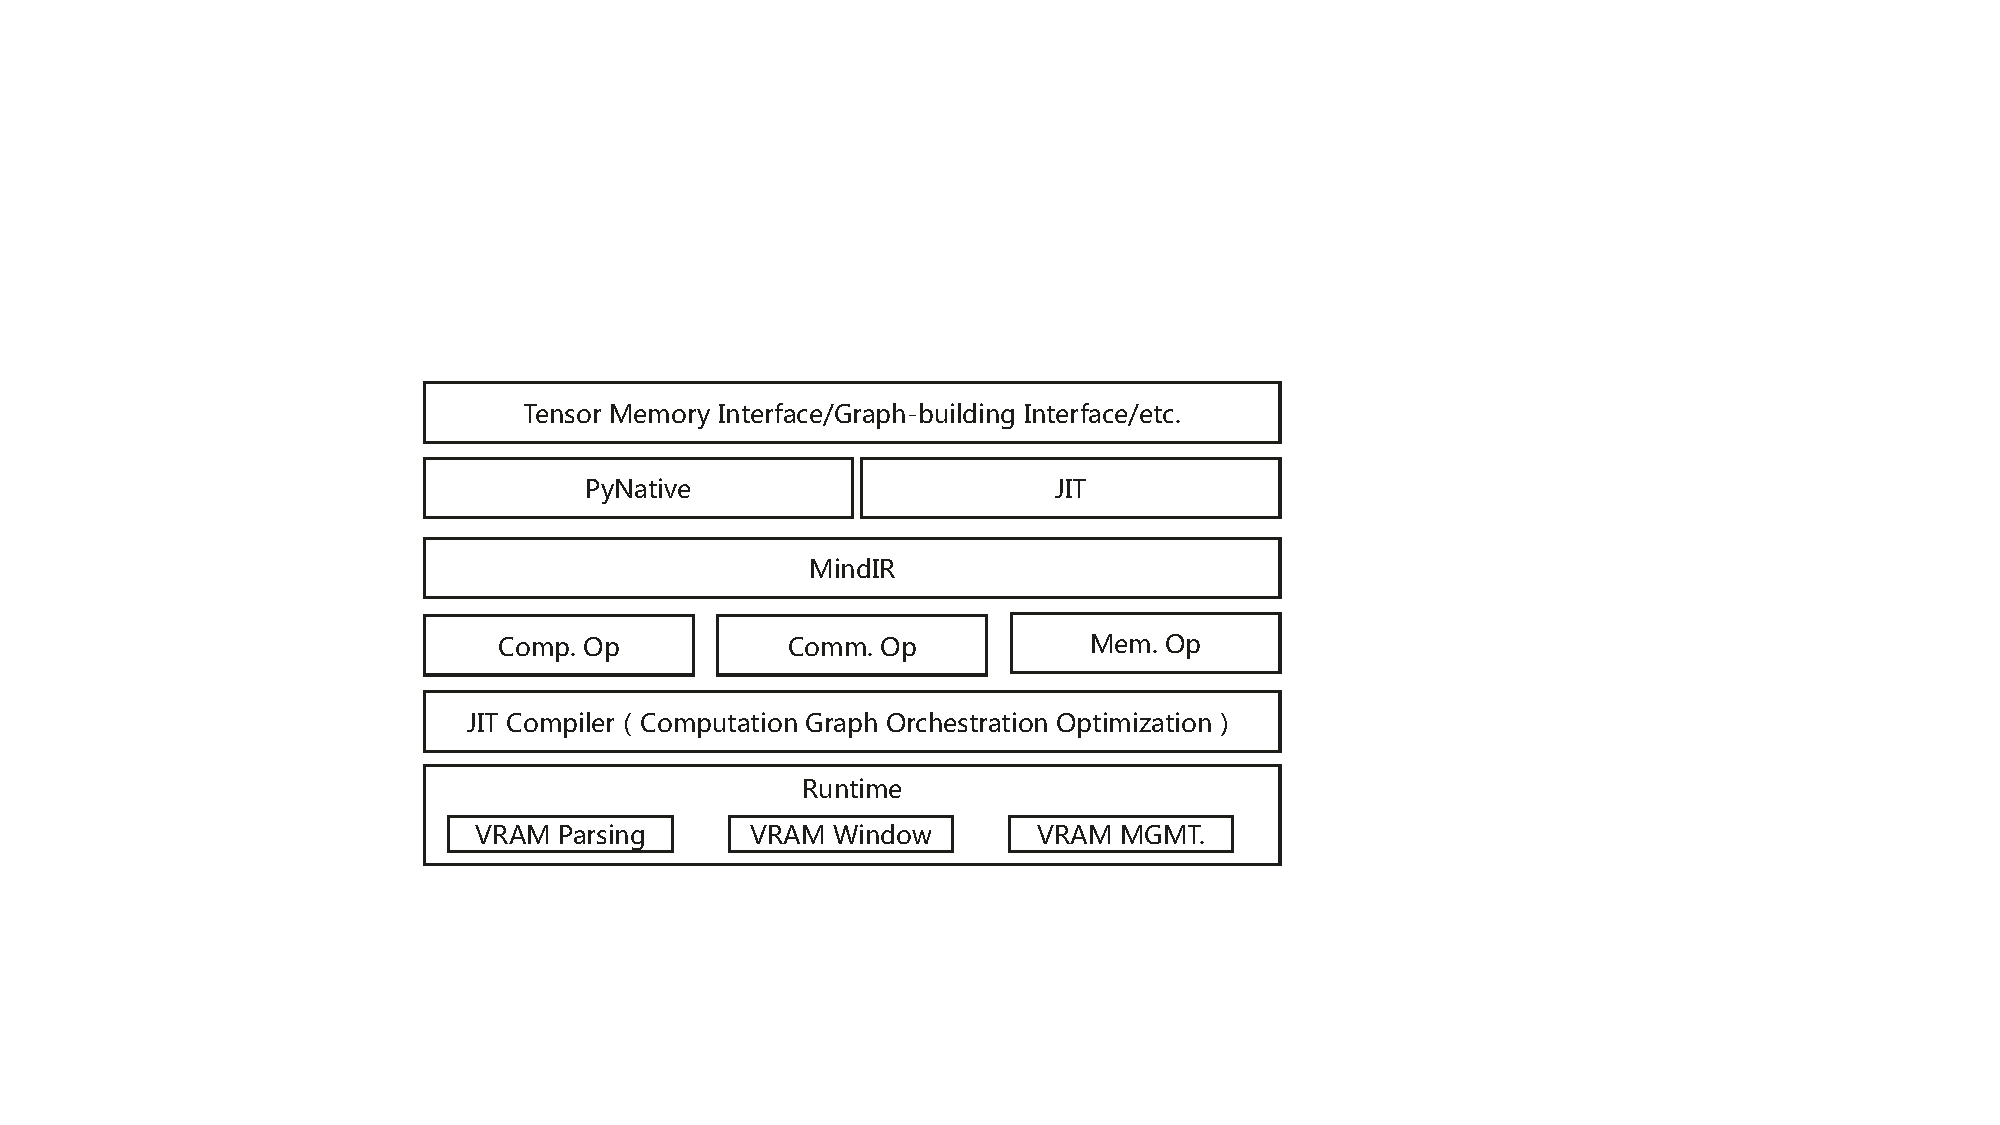
\includegraphics[width=0.7\linewidth]{figures/hyperoffload.pdf}
    \caption{\textit{HyperOffload}架构。}
    \label{fig:HyperOffload}
\end{figure}

\textbf{HyperOffload}的基本概念是将模型状态卸载到外部内存池，利用片上内存（HBM）作为高速缓存。这种架构允许单个加速器容纳显著更大的模型。核心挑战在于在不牺牲性能的情况下自动化HBM与DRAM之间的状态交换。为此，HyperOffload采用多级缓存流水线调度和全局图编排，如图~\ref{fig:HyperOffload}所示。

\begin{itemize}
    \item \textbf{多级缓存流水线调度} -- HyperOffload利用通信隐藏技术，在计算算子需要之前异步预取下一执行阶段所需的缓存块到高速存储层。通过将模型结构特性与数据访问模式预测相结合，系统动态调整预取路径，有效重叠加载延迟与计算时间。
    \item \textbf{全局图编排与调度} -- HyperOffload将分层缓存操作（如数据预取和块卸载）抽象为原生算子，实现缓存读写和迁移行为的统一描述。利用MindSpore的JIT图编译，框架在解析用户网络后自动插入缓存管理算子并重组执行流程。通过对缓存、计算和通信算子的统一编排，编译器自动调度并行执行链，消除了手动插入同步点的复杂性。
\end{itemize}

通过充分利用超节点的统一大内存池，HyperOffload显著放宽了训练和推理中的HBM内存约束。这使得可以去除复杂的$N$维SPMD并行，改用简单的1维SPMD数据并行，减少了状态同步的通信开销，进一步提升了性能。

实证结果表明了显著改进：
\begin{itemize}
    \item \textbf{训练场景} -- 在相同硬件配置下，Llama-8B模型每步迭代时间从传统方法的5.2s降至4.08s，性能提升约20\%。
    \item \textbf{推理场景} -- 在相同延迟限制下，HyperOffload将支持的序列长度从71K提升至123K，比传统方法提升70\%。
\end{itemize}

\subsection{HyperMPMD}

\begin{figure}
    \centering
    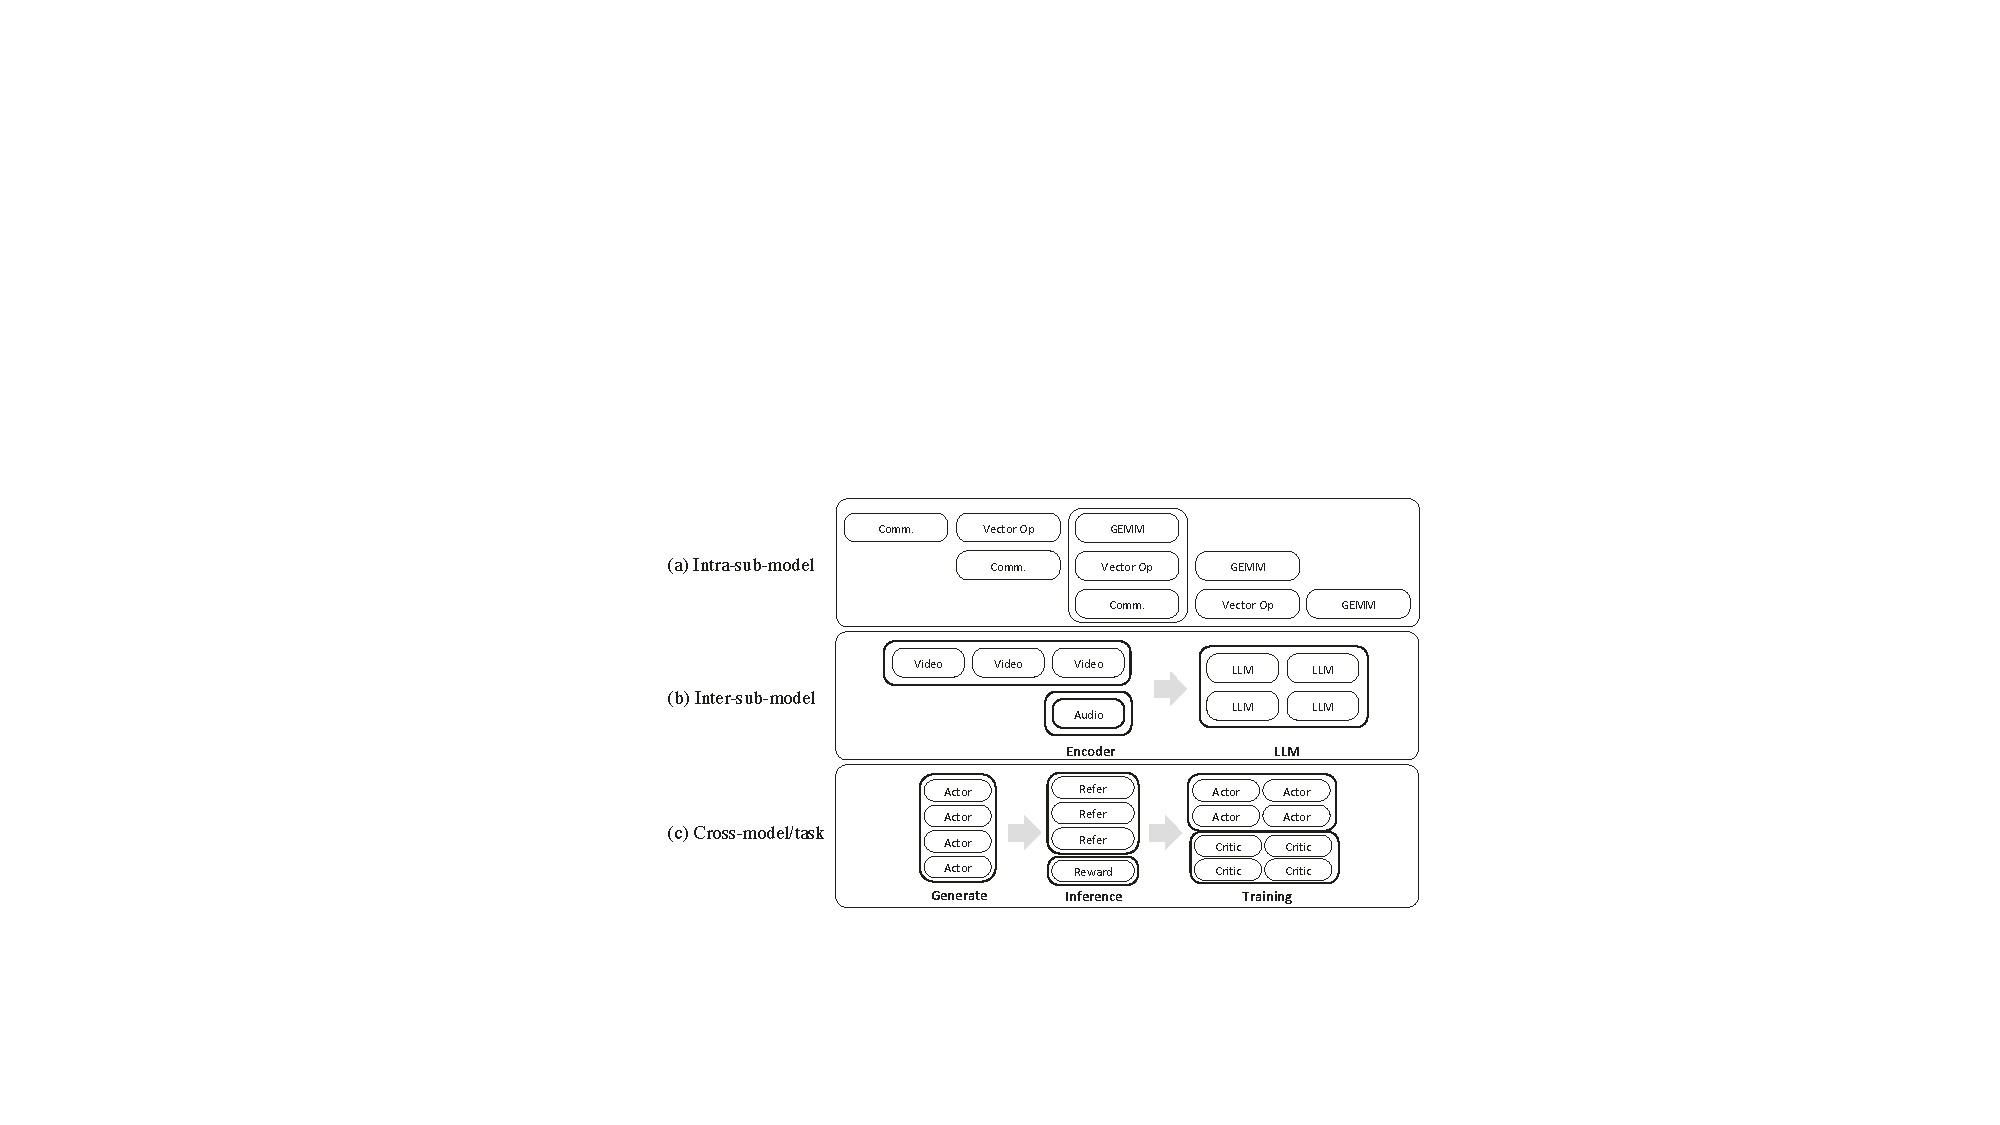
\includegraphics[width=\linewidth]{figures/hypermpmd.pdf}
    \caption{HyperMPMD示意图。}
    \label{fig:hypermpmd}
\end{figure}

\textbf{HyperMPMD}的核心目标是实现灵活、细粒度的多程序多数据（MPMD）分片方法，以解决全模态学习和强化学习等场景中的计算不均衡问题，从而最大化硬件利用率。HyperMPMD在三个不同维度上提供MPMD能力：

\begin{itemize}
    \item \textbf{子模型内AICube与AIVector级别的并发} -- 通过对模型张量进行分片，并利用卡内MPMD调度实现AICube和AIVector任务，框架实现了计算-通信重叠的细粒度编排（如图~\ref{fig:hypermpmd}(a)所示）。这解决了MoE架构中固有的通信掩盖挑战。通过协同卡内多核并行与卡间并行，HyperMPMD将通信掩盖率从传统的60\%提升至90\%。
    \item \textbf{子模型间并发均衡} -- 框架将子图解耦为独立的并发任务（如图~\ref{fig:hypermpmd}(b)所示），利用动态调度缓解负载不均衡。这有效消除了全模态或多模态模型中由异构子模块负载引起的10\%--40\%的流水线气泡，带来约15\%的整体训练性能提升。
    \item \textbf{跨模型并发调度} -- 与MPMD运行时集成，框架提供单一控制器（Single Controller）支持，在超节点池化计算资源内执行细粒度并行分片和动态调度（如图~\ref{fig:hypermpmd}(c)所示）。这实现了模型级并发，消除了落后者效应，解决了多任务强化学习中的负载不均衡，将全集群资源利用率提升了15\%。
\end{itemize}

HyperMPMD根据模态或任务（如文本、图像、音频、融合和任务调度组）划分独立的MPMD进程组。每个组执行专门的程序逻辑，通过标准化接口进行通信。以下示例展示了全模态MPMD进程组的配置。通过将核心逻辑封装到独立模块中，并通过代码清单~\ref{code:mpmd_config}中的配置文件定义\textit{节点到模块}的映射，框架消除了刚性硬编码的需求。

\begin{center}
\begin{minipage}{\textwidth}
\begin{lstlisting}[language=Python, caption={映射配置示例。}, label={code:mpmd_config}]
process_groups = {
  "text": {"ranks": [0,1], "module": TextModule, "hardware": "NPU"},
  "image": {"ranks": [2,3], "module": ImageModule, "hardware": "NPU"},
  "audio": {"ranks": [4], "module": AudioModule, "hardware": "CPU"},
  "fusion": {"ranks": [5], "module": CrossModalFusion, "hardware": "NPU"},
  "task_scheduler": {"ranks": [6], "module": TaskPriorityScheduler, 
                     "hardware": "CPU"}
}
\end{lstlisting}
\end{minipage}
\end{center}

\subsection{HyperShard}

\begin{figure}
    \centering
    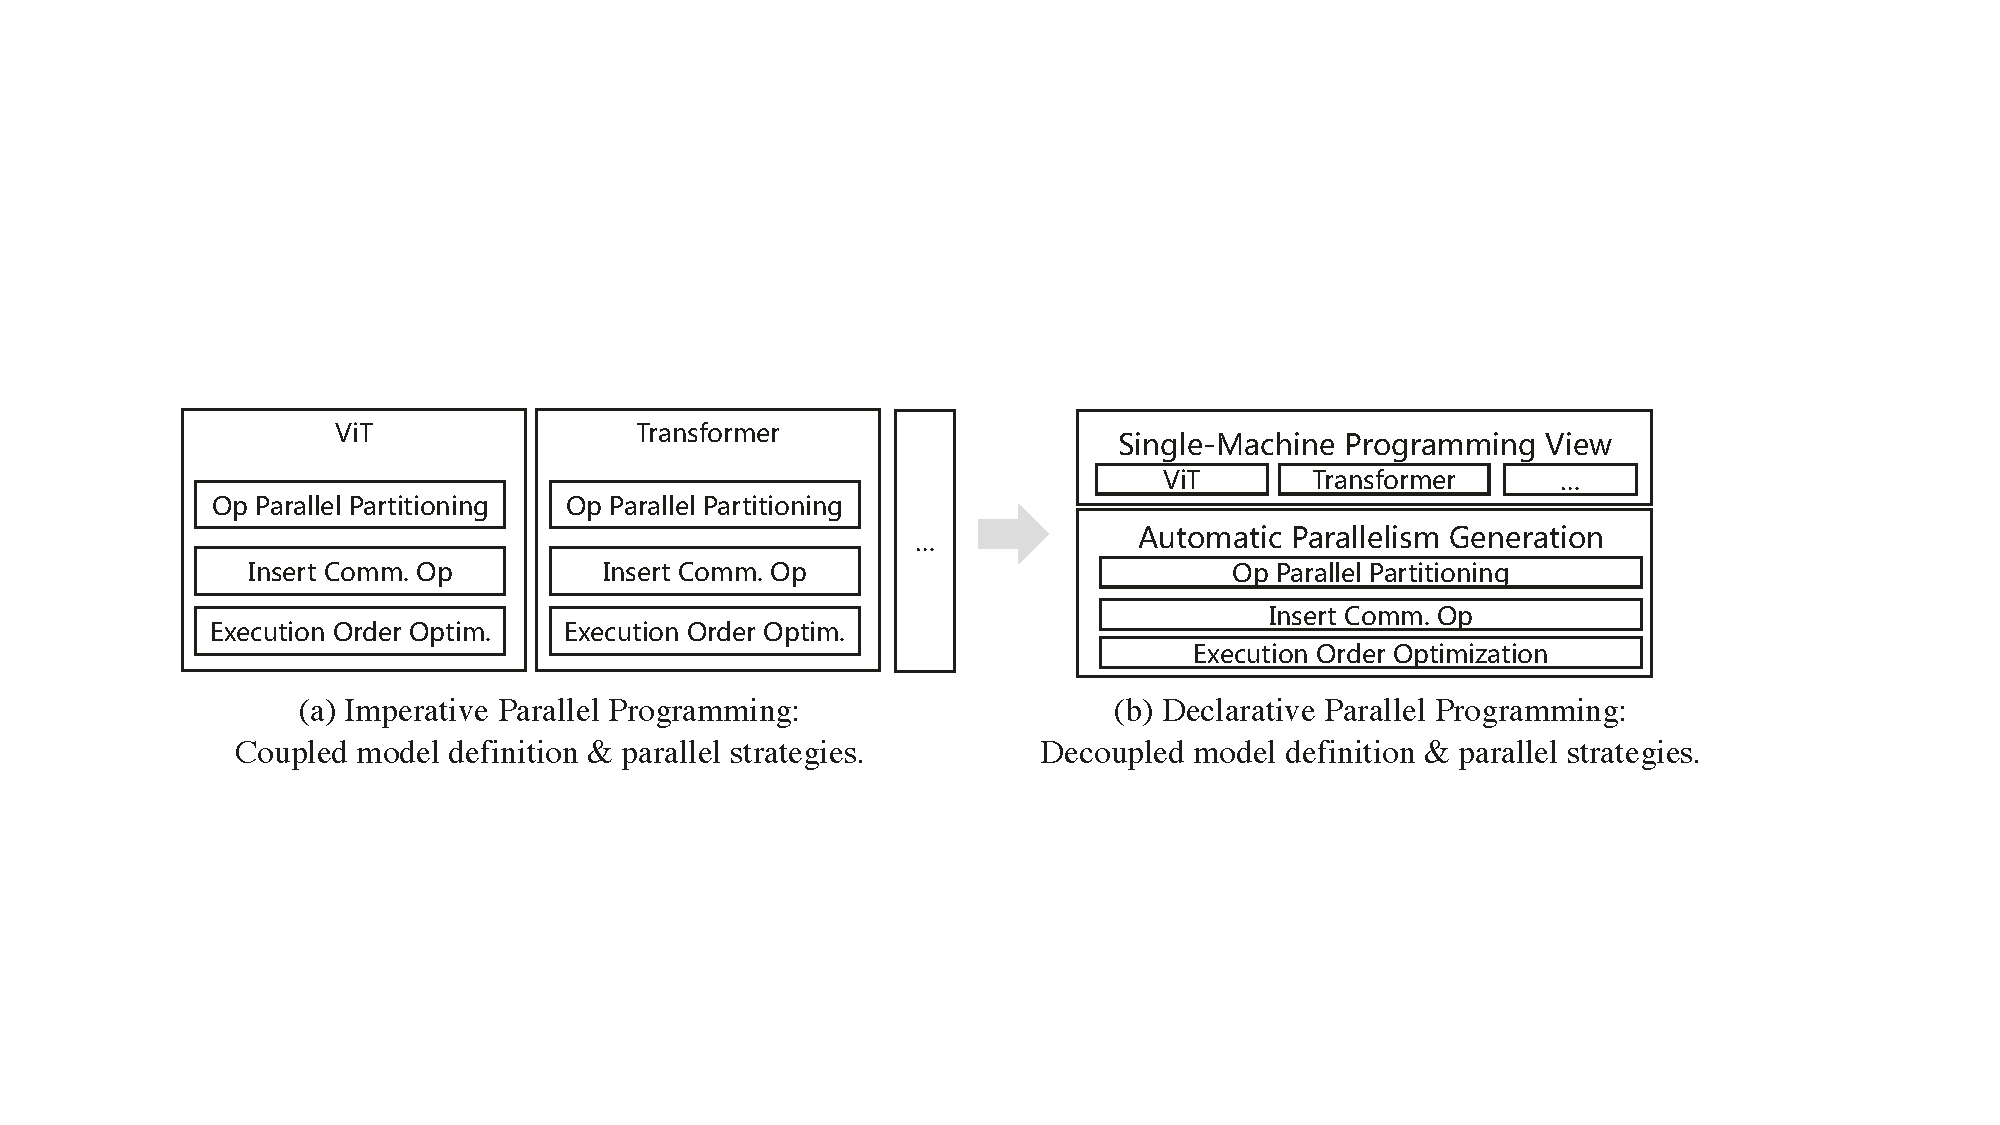
\includegraphics[width=\linewidth]{figures/declaritive_programming.pdf}
    \caption{声明式与命令式并行编程的比较。}
    \label{fig:comp_hypershard}
\end{figure}

\textbf{HyperShard}的基本目标是提供声明式并行编程能力，使开发者能够使用单节点编程规范构建模型，有效地将算法逻辑与并行策略解耦，允许后者根据网络拓扑灵活配置。如图~\ref{fig:comp_hypershard}(a)所示，传统的命令式并行编程存在模型定义与并行策略的紧密耦合问题，需要针对每个模型变体进行定制的手动干预——如算子分片、显式通信算子插入和执行序列优化。相比之下，图~\ref{fig:comp_hypershard}(b)展示了声明式范式：研究人员从单设备视角开发算法，仅声明所需的并行约束，框架随后自动生成底层并行策略，实现完全解耦。

\textbf{HyperShard}的主要编程抽象是接口\verb|Layout(device_matrix,| \verb|alias_name, tensor_map)|，定义如下：
\begin{itemize}
    \item \verb|device_matrix| -- 描述集群内加速器的逻辑排列。
    \item \verb|alias_name| -- 为设备矩阵内的每个维度分配描述性标识符。
    \item \verb|tensor_map| -- 指定给定张量的每个维度如何在设备矩阵上进行分区。
\end{itemize}

\begin{center}
\begin{minipage}{0.6\textwidth}
\begin{lstlisting}[language=Python,label={code:example_hypershard},caption=HyperShard策略生成示例。]
# 4个加速器组成2*2设备矩阵
device_matrix = (2, 2) 
# 设备矩阵每个维度的别名
alias_name = ("x", "y")
# 假设tensor.shape=(2, 2)
tensor_map = ("x", "y")
# 声明布局
layout = Layout(device_matrix, alias_name)
# 生成并行分区策略
parallel_strategy = layout(tensor_map)
\end{lstlisting}
\end{minipage}
\end{center}

以代码清单~\ref{code:example_hypershard}中的代码为例，我们展示在八个加速器上分片张量的过程。自动分片过程分三个阶段进行：
\begin{itemize}
    \item \textbf{图~\ref{fig:illus_Hypershard}(a)：初始化} -- 框架初始假设张量位于单个逻辑rank（如Rank 0）上。
    \item \textbf{图~\ref{fig:illus_Hypershard}(b)：第一维度分区} -- 由于\verb|tensor_map[0] = "x"|，框架沿\verb|device_matrix|的\verb|"x"|维度对张量的第0维进行分片。
    \item \textbf{图~\ref{fig:illus_Hypershard}(c)：第二维度分区} -- 由于\verb|tensor_map[1] = "y"|，框架沿\verb|device_matrix|的\verb|"y"|维度对张量的第1维进行分片。
\end{itemize}

关键需要注意的是，这一过程在编译时不涉及物理张量切片。相反，框架根据用户配置对并行策略（\textit{shard\_strategy}）进行形式化推导；实际的分片执行发生在运行时。

\begin{figure}
    \centering
    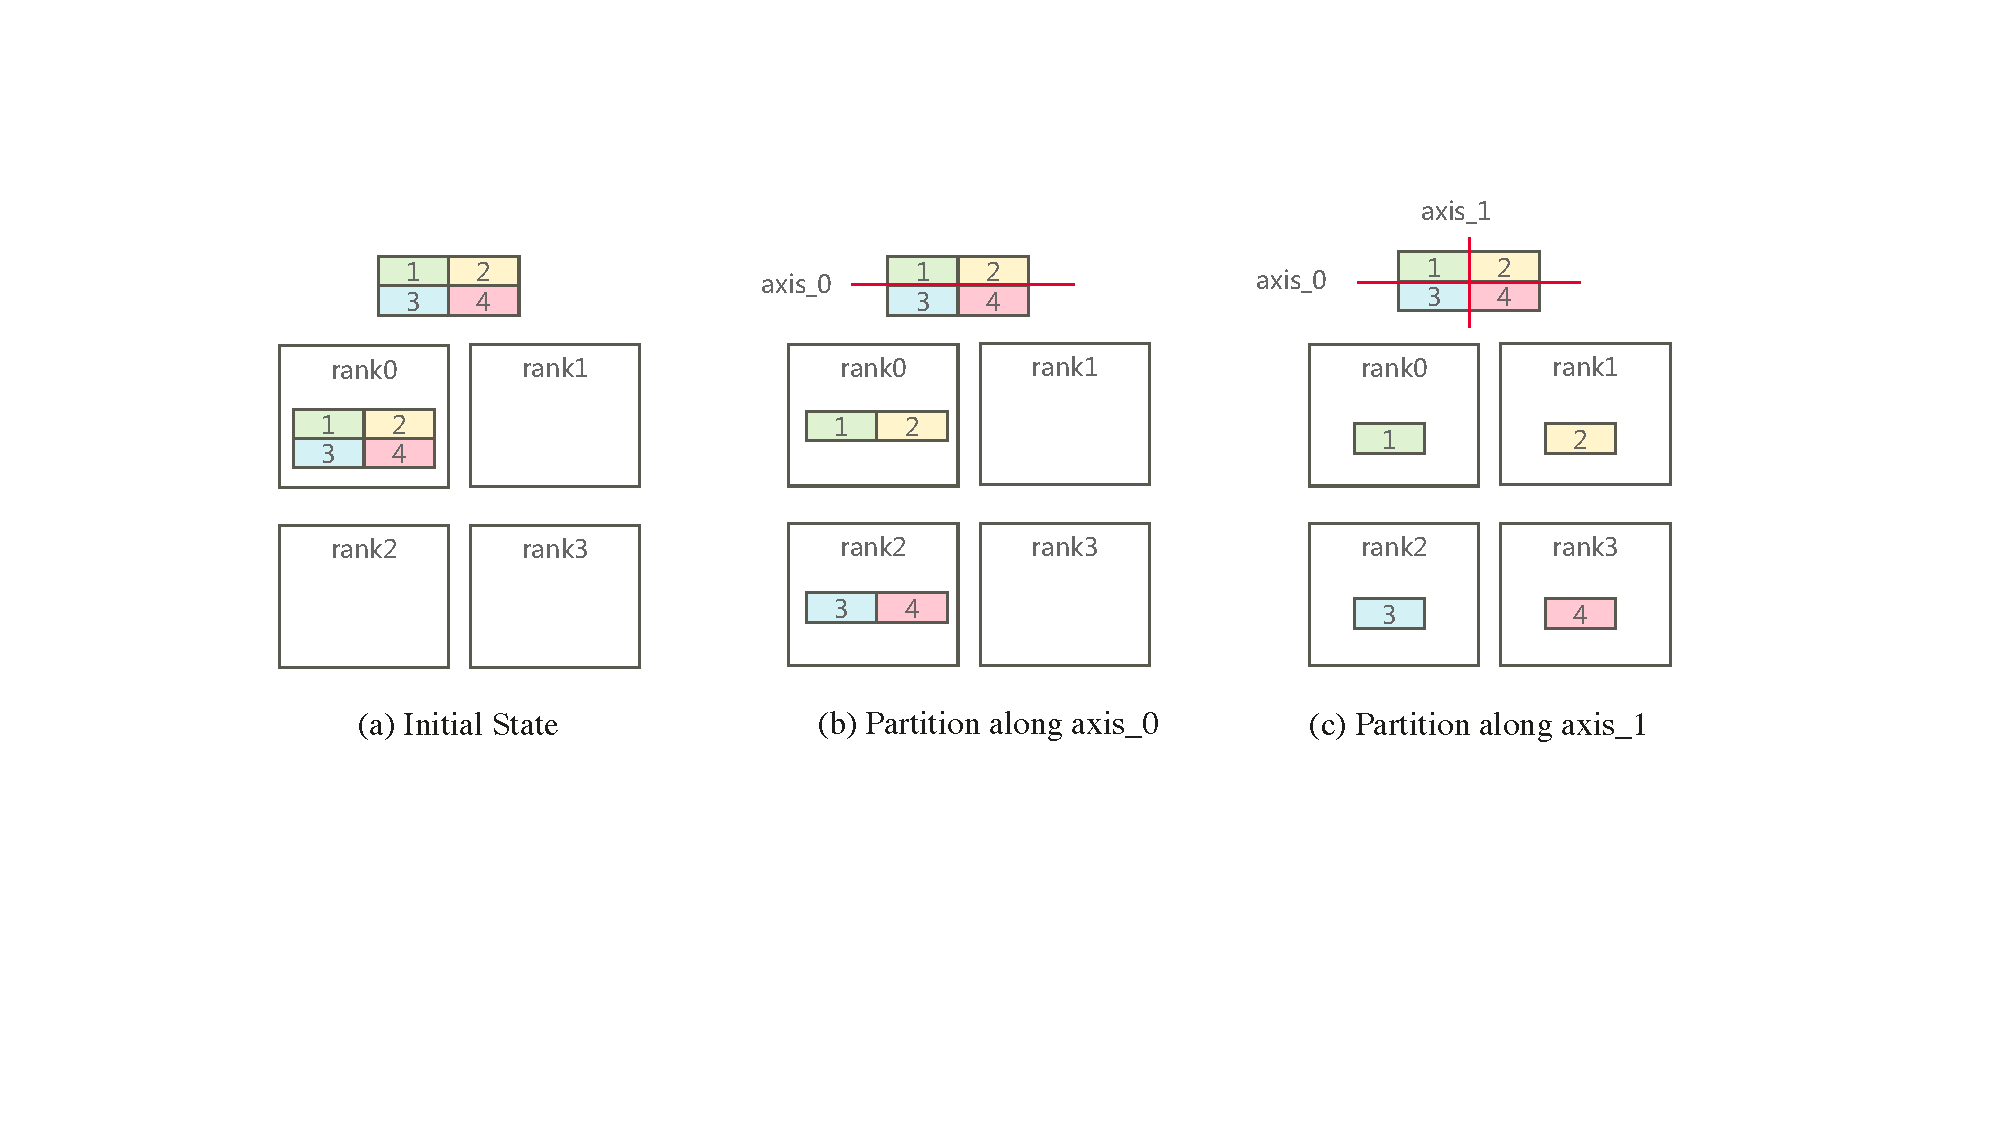
\includegraphics[width=1.0\linewidth]{figures/hypershard_partitioning.pdf}
    \caption{HyperShard分区示意图。}
    \label{fig:illus_Hypershard}
\end{figure}

通过将并行策略与算法解耦，屏蔽开发者的硬件复杂性，\textbf{HyperShard}显著降低了工程开销。新算法并行化所需的时间缩短至不到一天，并行策略优化周期从数天压缩至数小时。

\section{总结与讨论}
\label{sec5}
本文系统分析了模型工作负载、硬件架构和训练-推理范式的演进趋势，重点阐述了大规模模型和超节点集群对AI框架施加的挑战。我们识别了现有框架在并行分片、状态管理和集群利用率效率方面的关键不足，并提出了超节点亲和性AI框架的设计，基于MindSpore实现了\textbf{HyperParallel}架构。

通过三项核心技术——\textbf{HyperOffload}、\textbf{HyperMPMD}和\textbf{HyperShard}——的深度集成，框架实现了计算与状态的解耦、细粒度MPMD并行，以及声明式编程接口。这些创新带来以下贡献：

\begin{itemize}
    \item \textbf{复杂拓扑的抽象} -- 框架简化了开发和调优流程，使研究人员能够以与单节点编程相同的便利性开发大规模模型。
    \item \textbf{灵活高效的并行性} -- 通过提供动态细粒度的并行策略调度，框架最大化了超节点计算资源的利用率，有效解决了MoE、全模态和强化学习场景中的负载不均衡问题。
    \item \textbf{统一的状态管理} -- 利用统一内存池管理中间状态，提高了内存利用率，支持不断增大的模型的训练和推理而不损失性能。
\end{itemize}

实证结果表明，在相同硬件条件下，HyperOffload和HyperMPMD显著提升了训练和推理性能，同时大幅缩短了算法开发和并行策略优化所需的时间。展望未来，超节点亲和性AI框架可进一步扩展以支持异构任务调度、多节点动态扩展和跨数据中心协同训练，为下一代大规模模型研究和工业部署提供强大的软件基础设施。

\section{致谢}
我们诚挚感谢以下贡献者在HyperParallel框架开发中发挥的宝贵作用。

\noindent \textbf{研究与工程}

\noindent Changwei Ma,
Chao Fu,
Chen Li,
Chongming Liu,
Da Lei,
Dawei Fan,
Dongjie Geng,
Fuxin Huang,
Guangpeng Zhang,
Haoran Wang,
Huikang Tang,
Jiahong Qian,
Jiaqi Song,
Jinshan Ding,
Kaisheng Wang,
Mingqi Li,
Nuohang Li,
Qi Guo,
Qian Shu,
Renwei Zhang,
Shanni Li,
Xiangyu Meng,
Xinglei Xu,
Xiong Gao,
Yi Huang,
Yide Wang,
Yifan Yao,
Yixing Feng,
Zhenbang Wang,
Zheng Li,
Zhenzhang Yang,
Zherui Chang,
Zhibo Liang

\bibliographystyle{plain}
\bibliography{ref}

\end{document}
